\section{Forelesninger}

\subsection{Mandag \date{3. februar 2025}}

\paragraph{Von Neumann Stability Analysis}

\begin{itemize}
  \item Let \( U_m^n = \xi^n e^{i\beta m} \). Insert this into Difference Equation (DE).
  \item The method is Von Neumann Stable if \( \abs{\xi} \leq 1 + \mu K \) for all \( \beta \).
  \item Von Neumann stability is sufficient and necessary for pure IVP problems (Cauchy problems).
\end{itemize}
\begin{figure}[H]
  \centering
  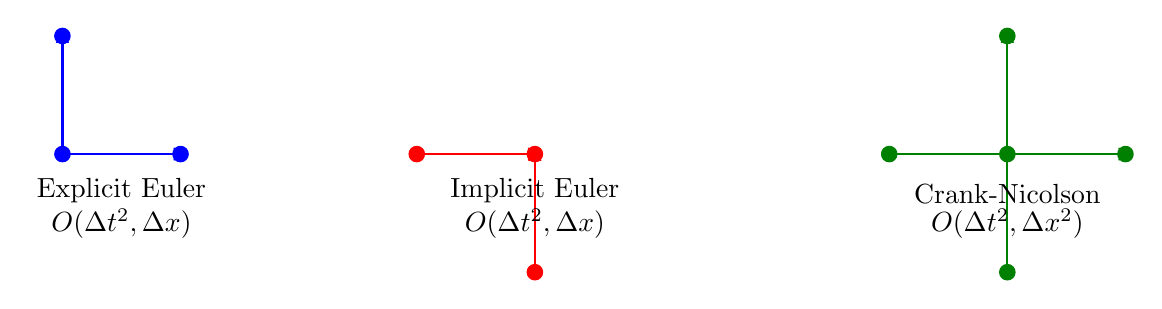
\begin{tikzpicture}[scale=1.5]
    % Explicit Euler (Forward)
    \begin{scope}[xshift=0cm]
      \fill[blue] (0,0) circle (2pt);
      \fill[blue] (0,1) circle (2pt);
      \fill[blue] (1,0) circle (2pt);
      \draw[->,thick,blue] (0,0) -- (1,0);
      \draw[->,thick,blue] (0,0) -- (0,1);
      \node[above] at (0.5,-0.5) {Explicit Euler};
      \node[above] at (0.5,-0.8) {\(O(\Delta t^2, \Delta x)\)};
    \end{scope}

    % Implicit Euler (Backward)
    \begin{scope}[xshift=4cm]
      \fill[red] (0,0) circle (2pt);
      \fill[red] (-1,0) circle (2pt);
      \fill[red] (0,-1) circle (2pt);
      \draw[->,thick,red] (-1,0) -- (0,0);
      \draw[->,thick,red] (0,-1) -- (0,0);
      \node[above] at (0,-0.5) {Implicit Euler};
      \node[above] at (0,-0.8) {\(O(\Delta t^2, \Delta x)\)};
    \end{scope}

    % Crank-Nicolson
    \begin{scope}[xshift=8cm]
      \fill[green!50!black] (0,0) circle (2pt);
      \fill[green!50!black] (1,0) circle (2pt);
      \fill[green!50!black] (-1,0) circle (2pt);
      \fill[green!50!black] (0,1) circle (2pt);
      \fill[green!50!black] (0,-1) circle (2pt);
      \draw[->,thick,green!50!black] (-1,0) -- (1,0);
      \draw[->,thick,green!50!black] (0,-1) -- (0,1);
      \node[above] at (0,-0.5) {Crank-Nicolson};
      \node[above] at (0,-0.8) {\(O(\Delta t^2, \Delta x^2)\)};
    \end{scope}
  \end{tikzpicture}
  \caption{Stencils for different numerical schemes}
  \label{fig:stencils}
\end{figure}



\begin{example}{Heat equation}{}
  \[
    u_t = u_{xx}, \quad 0 \leq x \leq 1, \quad 0 \leq t \leq 0.5
  \]
  \[
    \begin{cases}
      u(x, 0) = \sin(\pi x) \\
      u(0, t) = u(1, t) = 0
    \end{cases}
  \]
  \[
    u(x, t) = \sin(\pi x) e^{-\pi^2 t}
  \]

  \subparagraph{Finite Difference Scheme}
  \[
    \frac{1}{2k}\left( U_m^{n+1} - U_m^{n-1} \right) = \frac{1}{h^2}\left( U_{m-1}^n - 2U_m^n + U_{m+1}^n \right)
  \]

  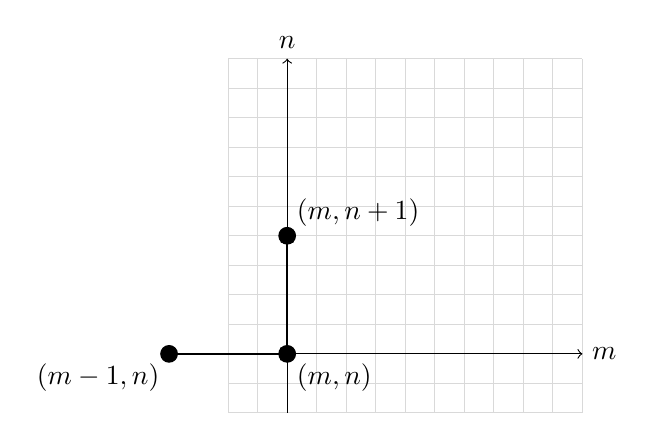
\begin{tikzpicture}[scale=1.5]
    % Grid
    \draw[step=0.25cm,gray!30] (-0.5,-0.5) grid (2.5,2.5);
    \draw[->] (-0.5,0) -- (2.5,0) node[right] {$m$};
    \draw[->] (0,-0.5) -- (0,2.5) node[above] {$n$};
    % Points
    \filldraw[black] (0,0) circle (2pt) node[below right] {$(m,n)$};
    \filldraw[black] (-1,0) circle (2pt) node[below left] {$(m-1,n)$};
    \filldraw[black] (0,1) circle (2pt) node[above right] {$(m,n+1)$};
    % Arrows
    \draw[->,thick] (0,0) -- (0,1);
    \draw[->,thick] (-1,0) -- (0,0);

  \end{tikzpicture}


  \subparagraph{Fourier Stability Analysis}

  \begin{align*}
    U_m^{n+1}
     & =
    2r\left( U_{m-1}^n - U_m^n + U_{m+1}^n \right) + U_m^{n-1}               \\
    \xi^{n+1} e^{i\beta x_m}
     & =
    2r\xi^n
    \left[
      e^{i\beta x_m - h} - 2e^{i\beta x_m} + e^{i\beta x_m + h}
      \right]
    + \xi^{n-1} e^{i\beta x_m}                                               \\
    \xi^2
     & =
    2r\left[ e^{-i\beta h} - 2 + e^{i\beta h} \right]\xi + 1                 \\
    \xi^2
     & =
    2r \left[ 2\cos(\beta h) - 2 \right]\xi+ 1                               \\
    \xi^2 + 8r\sin^2 \frac{\beta h}{2}\xi - 1
     & =
    0 \quad  \implies \quad \xi_\pm
    =
    -4r\sin^2 \frac{\beta h}{2} \pm \sqrt{16r^2\sin^4 \frac{\beta h}{2} + 1} \\
    \xi_- \leq - 1
    \quad
    \abs{\xi_-} \leq 1
  \end{align*}

  \textbf{Conclusion:} The scheme is unconditionally unstable.

  But we can stabilize the scheme by introducing a damping term (Du Fort-Frankel scheme):
  Replace \( U_m^n \leftarrow \frac{1}{2}(U_m^{n+1} + U_m^{n-1}) \) in the scheme.

  \begin{align*}
    \frac{1}{2k}\left( U_m^{n+1} - U_m^{n-1} \right)
     & =
    \frac{1}{h^2}\left( U_{m-1}^n + U_{m+1}^n\right) - \frac{1}{h^2}\left( U_m^{n+1} + U_m^{n-1} \right) \\
    (1 + 2r)U_m^{n+1}
     & =
    2r\left( U_{m-1}^n + U_{m+1}^n \right) + (1 - 2r)U_m^{n-1}                                           \\
    (1 + 2r)\xi^2 - 4r \cos \beta h \xi - (1 - 2r)
     & = 0                                                                                               \\
    \xi_\pm
     & = \frac{1}{1 + 2r} \left[ 2r\cos \beta h \pm \sqrt{4r^2\cos^2 \beta h + (1 - 2r)(1 + 2r)} \right] \\
    \xi_\pm
     & = \frac{1}{1 + 2r} \left[ 2r\cos \beta h \pm \sqrt{1 - 4r^2 \sin^2 {bh}} \right]                  \\
    \abs{\xi_\pm}^2 = \frac{2r - 1}{2r + 1} < 1 \quad \text{for all } r                                  \\
  \end{align*}

  \textbf{Conclusion:} The method scheme is unconditionally stable, for all \( r \).

  Now we know that the scheme has stability for all \( r \), it might still not converge because we also need consistency.

  \subparagraph{Consistency}
  \begin{align*}
    \tau_m^n
     & =
     & \frac{1}{2k}\left( u_m^{n+1} - u_m^{n-1} \right)                                                 \\
     & - \frac{1}{h^2}\left( u_{m-1}^n - u_{m+1}^n \right)                                              \\
     & + \frac{1}{h^2}\left( u_m^{n+1} - u_m^{n-1} \right)                                              \\
     & =
     & \frac{1}{2k}\left[ 2k u_t + 2k^3 \frac{1}{3!}u_{tt} + \ldots \right]                             \\
     & -\frac{1}{h^2}\left[ 2u + 2h^2 \frac{1}{2!}u_{xx} + 2h^4 \frac{1}{4!}u_{xxxx} + \ldots \right]   \\
     & + \frac{1}{h^2}\left[ 2 u + 2k^2 \frac{1}{2!}u_{tt} + 2k^4 \frac{1}{4!}u_{tttt} + \ldots \right] \\
     & =
    u_t - u_xx
    + \frac{k^2}{h^2}u_{tt} + \frac{k^2}{3!}u_{tt}
    + \frac{h^2}{12}u_{xxxx} + \frac{k^4}{12h^2}u_{tttt}
    + \ldots
  \end{align*}
  The method is consistent only if the truncation error goes to zero as \( h, k \to 0 \).

  Here the method is consistent when \(\frac{k}{h} \underset{h,k \to 0}{\longrightarrow} 0\).

  \textbf{Conclusion:} The method is conditionally consistent.

  \textbf{Conclusion:} The method is conditionally stable and consistent for all \( r \) and \( \frac{k}{h} \underset{h,k \to 0}{\longrightarrow} 0 \) and therefore convergent.

\end{example}

\paragraph{Domain of dependence}

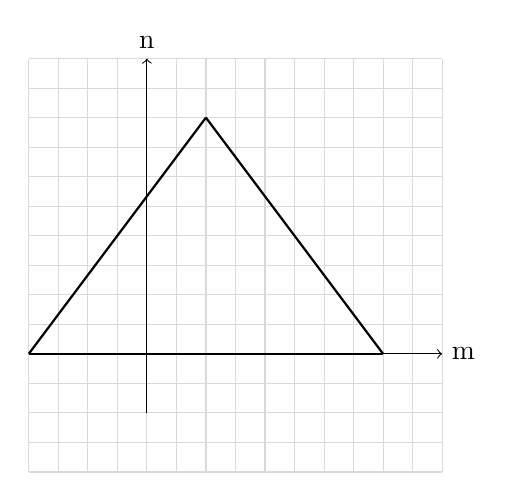
\begin{tikzpicture}[scale=1.5]
  % Grid
  \draw[step=0.25cm,gray!30] (-1,-1) grid (2.5,2.5);
  \draw[->] (-1,0) -- (2.5,0) node[right] {m};
  \draw[->] (0,-0.5) -- (0,2.5) node[above] {n};

  % Triangle
  \draw[-,thick] (-1,0) -- (0.5,2);
  \draw[-,thick] (-1,0) -- (2,0);
  \draw[-,thick] (2,0) -- (0.5,2);

\end{tikzpicture}


\subsection{Tirsdag \date{4. februar 2025}}

\paragraph{Hyperbolic PDEs}

\begin{align*}
  a u_{xx} + 2bu_{xy} + c u_{yy} = f(x,y, u, u_x, u_y) \tag{1} \\
  \begin{cases}
    b^2 - ac > 0 & \text{Hyperbolic} \\
    b^2 - ac = 0 & \text{Parabolic}  \\
    b^2 - ac < 0 & \text{Elliptic}
  \end{cases}                             \\
\end{align*}\label{eq:hb1}

\begin{example}{Wave equation}{}
  \begin{align*}
    u_{tt} & = c^2 u_{xx}                                                                                   \\
    u(x,0) & = f(x), \quad u_t(x,0) = g(x)                                                                  \\
    u(x,t) & = \frac{1}{2}\left[ f(x - ct) + f(x + ct) \right] + \frac{1}{2c} \int_{x-ct}^{x+ct} g(s) \, ds
  \end{align*}
\end{example}

\subparagraph{D'Alembert's principle}
\begin{figure}[H]
  \centering
  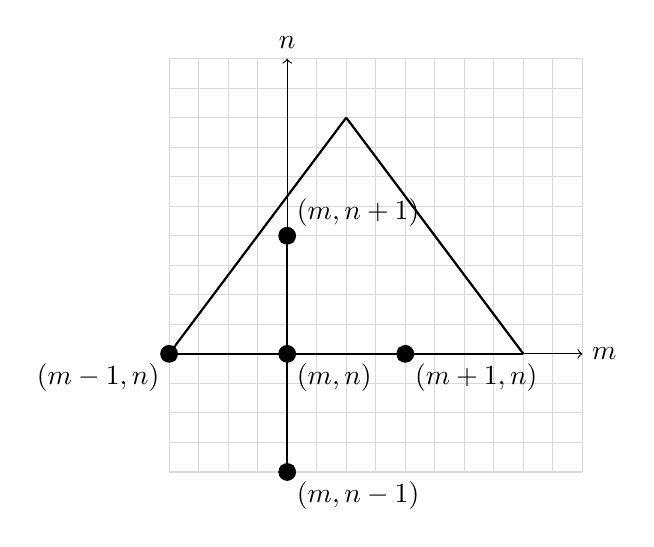
\begin{tikzpicture}[scale=1.5]
    % Grid
    \draw[step=0.25cm,gray!30] (-1,-1) grid (2.5,2.5);
    \draw[->] (-1,0) -- (2.5,0) node[right] {$m$};
    \draw[->] (0,-0.5) -- (0,2.5) node[above] {$n$};

    % Triangle
    \draw[-,thick] (-1,0) -- (0.5,2);
    \draw[-,thick] (-1,0) -- (2,0);
    \draw[-,thick] (2,0) -- (0.5,2);

    % Points
    \filldraw[black] (0,0) circle (2pt) node[below right] {$(m,n)$};
    \filldraw[black] (-1,0) circle (2pt) node[below left] {$(m-1,n)$};
    \filldraw[black] (0,1) circle (2pt) node[above right] {$(m,n+1)$};
    \filldraw[black] (1,0) circle (2pt) node[below right] {$(m+1,n)$};
    \filldraw[black] (0,-1) circle (2pt) node[below right] {$(m,n-1)$};

    % Arrows
    \draw[->,thick] (0,0) -- (0,1);
    \draw[->,thick] (0,0) -- (1,0);
    \draw[->,thick] (0,0) -- (-1,0);
    \draw[->,thick] (0,0) -- (0,-1);

  \end{tikzpicture}
  \caption{Stencils for the wave equation}
  \label{fig:wave-stencils}
\end{figure}

\begin{align*}
  Lu          & = \partial_t^2 u - c^2 \partial_x^2 u = (\partial_t - c \partial_x)(\partial_t + c \partial_x)u = 0 \\
  u_t + c u_x & = v                                                                                                 \\
  v_t - c v_x & = 0
\end{align*}

\subparagraph{1st order equations}
\begin{itemize}
  \item Density: \(u\)
  \item Non-conservative: \[ u_t + a(x,t,u)u_x = b(x,t,u) \tag{2} \]\label{eq:hb2}
  \item Transport equation: \(u_t + au_x = 0\) where \(a\) is a constant.
        \[
          \dd{t} \int_{x_1}^{x_2} u(x,t) \, dx = \int_{x_1}^{x_2} u_t(x,t) \, dx = -\int_{x_1}^{x_2} (f(u))_x \, dx = f(u(x_1,t)) - f(u(x_2,t))
        \]
  \item Conservation laws: \(u_t + (f(u))_x = 0\)
\end{itemize}

\subparagraph{1st order system}
\begin{itemize}
  \item Non-conservative: \[\symbf{u_t} + A(\symbf{u}_x) = \symbf{b}\tag{3}\]\label{eq:hb3}
  \item Conservative: \[\symbf{u_t} + (\symbf{f}(\symbf{u}))_x = 0\]
        This is hyperbolic if \(A\) is diagonalizable with real eigenvalues.
        \[
          A = PDP^{-1} \quad \text{where} \quad D = \text{diag}(\lambda_1, \ldots, \lambda_n)
        \]
        Equivalently, if the Jacobian matrix of \(\symbf{f}\) is diagonalizable with real eigenvalues.

        For linear problems (Hyperbolic PDEs),\eqref{eq:hb1} can always be written as \eqref{eq:hb3}.
        \eqref{eq:hb3} can always be decoupled into a set of \eqref{eq:hb2} equations.
\end{itemize}
\paragraph{Method of Characteristics}
Let \(u_t + a(x,t,u)u_x = b(x,t,u)\) be a non-conservative hyperbolic PDE. Furthermore let \(v(t) = u(x(t), t)\) where \(x(t)\) is a characteristic curve. Then
\[
  \dot{v} = u_x \dot{x} + u_t = u_t + a(x,t,u)u_x = b(x(t), t, u(x(t), t)=v(t))
\]
Let \(\dot{x} = a(x,t,u)\) (characteristic equation) and \(\dot{v} = b(x(t), t, v(t))\) (System of ODEs).
Initial values: \(\begin{cases} x(t_0) = x_0 \\ v(t_0) = u(x_0, t_0) \end{cases}\) is known for all \((t_0, x_0)\) on the initial curve.

\begin{align*}
  x(t) & = \mathcal{X}(t; t_0, x_0), \quad x_0 = x(t_0) = \mathcal{X}^{-1}(x, t)               \\
  v(t) & = \mathcal{V}(t; x_0, t_0, u_0), \quad u(x,t) = \mathcal{V}(t, \mathcal{X}^{-1}(x,t))
\end{align*}

\begin{example}{\(u_t + a u_x = b\) where \(a, b\) can be functions of \(x, t, u\)}{}
  \begin{align*}
    u_t + a(x,t,u)u_x & = b(x,t,u)                                                                                                          \\
    u(x,0)            & = u_0(x)   \quad \Sigma \text{ is the initial curve}                                                                \\
    \dot{x(t)}        & = a, \quad x(0) = x_0 \implies x(t) = x_0 + at \implies x_0 = x - at \implies u(x_0, 0) = u_0(x_0) \text{ is known} \\
    \dot{v(t)}        & = b
  \end{align*}

  % FYLL FRA BILDER PÅ TLF!

\end{example}


\subparagraph{Finite Difference Scheme}
\[
  \frac{1}{k^2}\left( U_m^{n+1} - 2U_m^n + U_m^{n-1} \right) = \frac{1}{h^2}\left( U_{m-1}^n - 2U_m^n + U_{m+1}^n \right)
\]

\subparagraph{Von Neumann Stability Analysis}
\begin{align*}
  U_m^n         & = \xi^n e^{i\beta m}                                                    \\
  \xi^2         & = \frac{1}{r^2} - 2 + \frac{1}{r^2} = 2\left( \frac{1}{r^2} - 1 \right) \\
  \xi_\pm       & = \pm \sqrt{2\left( \frac{1}{r^2} - 1 \right)}                          \\
  \abs{\xi_\pm} & \leq 1 \quad \text{if} \quad r \geq 1
\end{align*}

\textbf{Conclusion:} The method is conditionally stable.

\subparagraph{Consistency}
\[
  \tau_m^n = \frac{1}{k^2}\left( u_t - u_{xx} \right) + O(k^2, h^2)
\]

\textbf{Conclusion:} The method is consistent.

\textbf{Conclusion:} The method is conditionally stable and consistent and therefore convergent.


\begin{example}{}{}

  \[
    u_t + e^{-x}u_x = 0, \quad u(x,0) = u_0(x)
  \]

  \textbf{Method of Characteristics:}
  \begin{align*}
    \dot{x} & = e^{-x}, \quad x(0) = x_0             \\
    \dot{v} & = 0, \quad v(0) = u(x_0, 0) = u_0(x_0)
  \end{align*}
  \begin{align*}
    \frac{dx}{dt} = e^{-x} & \implies \int_{x_0}^x e^x \, dx = \int_0^t \, dt \implies e^x - e^{x_0} = t \implies x_0 = \ln(e^x - t) \\
    \frac{dv}{dt} = 0      & \implies v = u_0(x_0) = u_0(\ln(e^x - t))
  \end{align*}

\end{example}


\subsection{Onsdag \date{10. februar 2025}}

\paragraph{What about systems?}

\begin{align*}
  \symbf{u_t} + A(\symbf{u}_x)                           & = \symbf{0} \\
  \symbf{u_t} + P\Lambda P^{-1}(\symbf{u}_x)             & = \symbf{0} \\
  P^{-1}\symbf{u_t} + \Lambda P^{-1}\Lambda(symbf{u}_x) & = \symbf{0} \\
  \symbf{v_t} + \Lambda \symbf{v}_x                      & = \symbf{0}
\end{align*}

Hyperbolic if \(A\) is diagonalizable with real eigenvalues: \(A = P\Lambda P^{-1}\) where \(\Lambda = \text{diag}(\lambda_1, \ldots, \lambda_n)\).

\begin{example}{}{}
  \begin{align*}
    \symbf{v_{i,t} + \lambda_i v_{i,x} = 0}                                  \\
    \symbf{u}_t +
    \begin{bmatrix}
      a & b \\
      c & d
    \end{bmatrix}
    \symbf{u}_x = \symbf{0} \quad \text{where} \quad x\in [0,1], \quad t \geq 0 \\
    \symbf{u}(x,0) = \symbf{f}(x) \quad \text{is the initial curve}
  \end{align*}

  Then the eigenvalues are \(\lambda_{1,2} = a \pm b\) with eigenvectors
  \[
    P = \begin{bmatrix}
      1 & 1  \\
      1 & -1
    \end{bmatrix}
  \]
  and
  \[
    \symbf{v} = P^{-1}\symbf{u} \implies \symbf{u} = P\symbf{v}
  \]

  then we get the system

  \begin{align*}
    \symbf{v}_{1,t} + (a + b)\symbf{v}_{1,x} & = 0 \\
    \symbf{v}_{2,t} + (a - b)\symbf{v}_{2,x} & = 0
  \end{align*}

  assume that \(a > 0\), with the BCs
  \[
    x=0 \quad \text{inflow if } \lambda > 0 \quad \vee quad x = 1 \quad \text{outflow if } \lambda < 0
  \]

  \subparagraph{Case 1}
  \[
    a > b \quad \text{and} \quad \lambda_1, \lambda_2 > 0
  \]



\end{example}


\paragraph{Scheming}
\[
  \symbf{u}_t + a \symbf{u}_x = 0 , \quad b \in \R \quad \symbf{u}(x,0) = \symbf{f}(x)
\]

%draw Grid
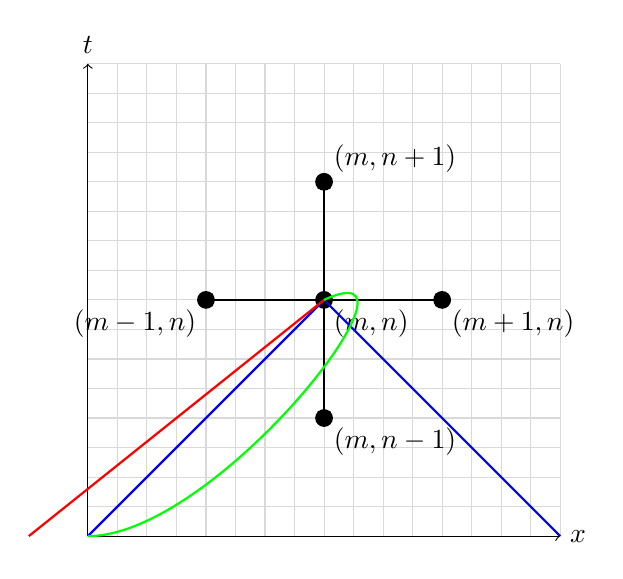
\begin{tikzpicture}[scale=1.5]
  % Grid
  \draw[step=0.25cm,gray!30] (-1,-1) grid (3,3);
  \draw[->] (-1,-1) -- (3,-1) node[right] {$x$};
  \draw[->] (-1,-1) -- (-1,3) node[above] {$t$};

  % Points
  \filldraw[black] (1,1) circle (2pt) node[below right] {$(m,n)$};
  \filldraw[black] (0,1) circle (2pt) node[below left] {$(m-1,n)$};
  \filldraw[black] (1,2) circle (2pt) node[above right] {$(m,n+1)$};
  \filldraw[black] (2,1) circle (2pt) node[below right] {$(m+1,n)$};
  \filldraw[black] (1,0) circle (2pt) node[below right] {$(m,n-1)$};

  % Stencils
  \draw[->,thick] (1,1) -- (1,2);
  \draw[->,thick] (1,1) -- (2,1);
  \draw[->,thick] (1,1) -- (0,1);
  \draw[->,thick] (1,1) -- (1,0);

  % Stencil 2 (Orange)
  \draw[-,thick,blue] (-1,-1) -- (1,1);
  \draw[-,thick,blue] (3,-1) -- (1,1);

  % Stencil 3 (red, outside)
  \draw[-,thick,red] (-1.5,-1) -- (1,1);

  % Stencil 4 (green, curved inside)
  \draw[-,thick,green] (-1,-1) to [out=0,in=25] (1,1);



\end{tikzpicture}

\subparagraph{Central Time, Central Space}
\[
  \frac{1}{k}\left( U_m^{n+1} - U_m^{n-1} \right) = \frac{1}{h}\left( U_{m+1}^n - U_{m-1}^n \right)
\]

\subparagraph{Forward Time, Central Space}
\[
  \frac{1}{k}\left( U_m^{n+1} - U_m^n \right) = \frac{1}{h}\left( U_{m+1}^n - U_{m-1}^n \right)
\]

´
Then
\[
  U_m^{n+1} = \beta_{-1} U_{m-1}^n + \beta_0 U_m^n + \beta_1 U_{m+1}^n
\]

Assume that \(\beta_{-1} \neq 0\) and \(\beta_1 \neq 0\), then the method is unconditionally unstable.

\begin{align*}
  T = k n                                                     \\
  x_{m-n} = \mathcal{X} - \dfrac{T}{k}h = \mathcal{X} - \mu T \\
  x_{m+n} = \mathcal{X} + \dfrac{T}{k}h = \mathcal{X} + \mu T
\end{align*}

Interval of dependence: \(\left[ \mathcal{X} - \mu T, \mathcal{X} + \mu T \right]\)

Domain of dependence: Triangle of this and \((X,T)\).

\subparagraph{Characteristics}

\begin{align*}
  x = x_0 + at \implies x_0 = x - at \quad \text{goes through} \quad (\mathcal{X}, T) \\
  x_0 = \mathcal{X} - \mu T \quad \text{CFL condition} \\
  \text{We need} \quad x_0 = \mathcal{X} - \mu T \in [X - \mu T, X + \mu T] \\
  \abs{a} \frac{k}{h} \leq 1 \quad \text{CFL condition}
\end{align*}

\subparagraph{Forward Time, Backward Space}
\[
  \frac{1}{k}\left( U_m^{n+1} - U_m^n \right) = a \frac{1}{h}\left( U_m^n - U_{m-1}^n \right)
\]

Let \(p = a \frac{k}{h}\), then

\[
  U_m^{n+1} = U_m^n + p(U_{m-1}^n - U_m^n)
\]

\subparagraph{Von Neumann Stability Analysis}
\[
  U_m^n = \xi^n e^{i\beta m} \quad \beta \in \R
\]

Stable if there is a \(\mu> 0\) such that \(\abs{\xi} \leq 1 + \mu k \).

For the FTBS scheme, we get

\begin{align*}
  \xi^{n+1} e^{i\beta m} & = \xi^n e^{i\beta m} + p\xi^n\left( e^{i\beta m} - e^{i\beta (m-1)} \right) \\
  \xi                   & = 1 - p(1 - e^{-i\beta h}) = (1 - p) + pe^{-i\beta h}                            \\
\end{align*}

Here we can see that \(\abs{\xi} \) is just a circle in the complex plane with radius \(p\) and center \((1-p)\).

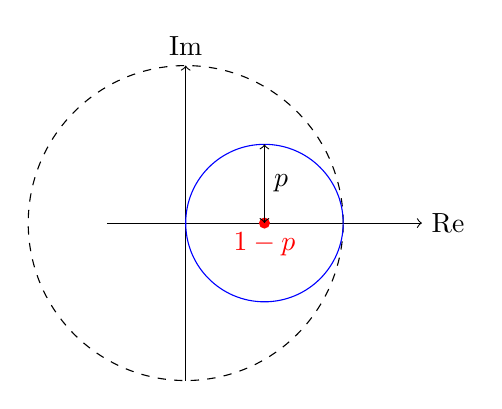
\begin{tikzpicture}[scale=2]
  % Parameters
  \def\p{0.5}

  % Axes
  \draw[->] (-0.5,0) -- (1.5,0) node[right] {Re};
  \draw[->] (0,-1) -- (0,1) node[above] {Im};
  
  % Unit circle
  \draw[dashed] (0,0) circle (1);
  
  % Circle representing xi
  \draw[blue] (1-\p,0) circle (\p);
  
  % Center point
  \fill[red] (1-\p,0) circle (1pt) node[below] {$1-p$};
  
  % Radius label
  \draw[<->] (1-\p,0) -- ++(0,\p) node[midway,right] {$p$};
\end{tikzpicture}

So the scheme is stable if \(\abs{\xi} \leq 1 \) if \(0 < p \leq 1\) or \(0 < a \frac{k}{h} \leq 1\).

What happens if we have \(a < 0\)? In this case the condition \(\abs{\xi} \leq 1 \) for all \( \beta \) is not satisfied.

\subparagraph{Forward Time, Central Space}

\[
  U_m^{n+1} = U_m^n - \frac{p}{2}\left( U_{m+1}^n - U_{m-1}^n \right)
\]

Then we get the stability condition:

\begin{align*}
  \xi & = 1 - \frac{p}{2}\left( e^{i\beta h} - e^{-i\beta h} \right) = 1 - p\sin(\beta h) \\
  \abs{\xi} & = \sqrt{(1 - p\sin^2(\beta h))} = 1 - p\sin(\beta h) \leq 1
\end{align*}



